\section{Experiments}
\label{sec:experiments}

The parameter space for the hidden states, the associated prior $H$ on
$\btheta$, and the similarity function
$\Phi$, is application-specific; we consider here the case where a state
consists of a finite $D$-dimensional binary vector, $\eta_j$, the similarity
function is a Laplacian kernel defined with respect to Hamming
distance between pairs $\eta_j$ and $\eta_{j'}$ with decay parameter
$\lambda$, and the emission distribution is linear-Gaussian, with $D
\times K$ weight matrix $\bW$, so that each $K$-dimensional
observation is $\Norm{\bW \eta_j}{\Sigma}$.  For experiments discussed
here, we will assume that $\Sigma$ does not depend on $j$, but this assumption
is easily relaxed if appropriate.  For finite-length binary vector
states, the set of possible states is finite, and so on its face it may
seem that a nonparametric model is unnecessary.  However, if $D$ is
reasonably large, it is likely that most of the $2^D$ possible states
are vanishingly unlikely (and, in fact, the number of observations may
well be less than $2^D$), and so we would like a model that encourages
the selection of a sparse set of states.  Moreover, there could be more
than one state with the same emission parameters, but with different transition
dynamics.  Before describing individual experiments, we describe the additional
inference steps needed for these variables.

\subsection{Additional Inference Steps}
\label{sec:sampling-eta}

\paragraph{Sampling $\eta$} We put independent Beta-Bernoulli priors
on each coordinate of $\eta$.  We Gibbs sample each coordinate $\eta_{jd}$
conditioned on all the others and the coordinate-wise prior means,
$\{\mu_d\}$, which we sample in turn conditioned on the $\eta$s.

\paragraph{Sampling \texorpdfstring{$\lambda$}{kernel decay rate}}
\label{sec:sampling-lambda}
The Laplacian kernel $\Phi$ is defined as $\Phi(\eta_j, \eta_{j'}) =
e^{-\lambda d(\eta_j,\eta_{j'})}$, where in our case $d$ is
  Hamming distance.  The parameter $\lambda$ governs the connection between $\btheta$ and
$\bphi$.  Writing \eqref{eq:65} in terms of $\lambda$ and the distance matrix
$\boldsymbol{\Delta}$ gives the likelihood
\begin{equation}
  \label{eq:88}
  p(\bz, \bQ \given \lambda, \btheta) \propto \prod_{j}\prod_{j'}
  e^{-\lambda \Delta_{jj'} n_{jj'}}(1-e^{-\lambda\Delta_{jj'}})^{q_{jj'}} 
\end{equation}
We put an $\Exp{b_{\lambda}}$ prior on $\lambda$, which yields a
posterior density
\begin{equation}
  \label{eq:88}
  p(\lambda \given \bz, \bQ, \btheta) \propto
  e^{-(b_{\lambda} + \sum_{j}\sum_{j'} \Delta_{jj'} n_{jj'})\lambda} \prod_{j}\prod_{j'}
  (1-e^{-\lambda\Delta_{jj'}})^{q_{jj'}}
\end{equation}
This density is log-concave, and so we use Adaptive Rejection Sampling \cite{gilks1992adaptive}
to sample from it.

\paragraph{Sampling \texorpdfstring{$\bW$}{weights} and
  \texorpdfstring{$\Sigma$}{emission covariance}}
Conditioned on the state matrix $\btheta$ and the data matrix $\bY$, 
the weight matrix $\bW$ can be sampled as well using standard methods
for Bayesian linear regression.  We place a zero mean Normal prior on each
element of $\bW$ (including a row of intercept terms), resulting in a
multivariate Normal posterior for each column.  For the experiments
reported below, we constrain $\Sigma$ to be a diagonal matrix, and
place an Inverse Gamma prior on the variances, resulting in conjugate updates.

\subsection{``Cocktail Party'' Data}

To evaluate the model, we created synthetic data based on a speaker 
diarization task, with the property that speakers are grouped into
conversations, and take turns speaking within conversation.   
In such a task, there are naively $2^S$ possible
states, where each state indicates which of $S$ speakers is speaking
at a particular time step.  However, due to the conversational grouping, if
at most one speaker in a conversation can be speaking at any given
time (a natural assumption of within-group turn-taking), 
the state space is constrained, with only $\prod_c (s_c + 1)$
states possible, where $s_c$ is the
number of speakers in conversation $c$.

For the cocktail party data, the turn sequence within conversations is
generated using a Poisson HSMM with $s_c$ states, with pauses with
shorter Poisson duration inserted between each ``sentence''.  The
states within conversations were then mapped to a binary vector with
$s_c$ entries, where silence is represented by all zeroes, 
and speaker $s$ speaking corresponds to
a 1 in position $s$.  The binary vectors were concatenated across
conversations to yield latent states consisting of length $S$ binary
vectors.  To simulate speakers being recorded by $K$ microphones,
weights from speakers to microphones were generated independently from
a $U(0,1)$ distribution, resulting in a $D \times K$ weight matrix,
$\bW$.  A constant ``background sound level'' parameter for each microphone was added as
well, also $U(0,1)$, and independent $\Norm{0}{\sigma^2_k}$ noise was added
to each time step at microphone $k$.

We generated transition and emission parameters from conjugate priors
to the Poisson HSMM.  The data set
consisted of four conversations of four speakers each, and 12
microphones, so that $D = 16$, and $K = 12$.  There are therefore
$2^{16} = 65536$ possible binary vector-valued states, but only
$(4+1)^4 = 625$, less than 1\%, can actually occur.  The noise variance $\sigma^2_k$ 
was set to a constant of $1/10$ for all $k = 1, \dots, K$.

We attempted to infer the states
from the data using three models: (1) a binary-state Factorial HMM, in which the
individual binary speaker sequences are modeled as independent a
priori, (2) an ordinary HDP-HMM without local transitions, where the
latent states are binary vectors, and (3) our
HDP-HMM-LT model.  To simplify interpretation of the results, the weight matrix
was fixed to the true value (this makes the latent dimensions
identifiable and makes distances between inferred and ground truth
state matrices meaningful).  We evaluated the models at each
iteration using Hamming distance between inferred 
and ground truth state matrices and F1 score.
The results for the three models are in Figure
\ref{fig:cocktail-results}.  % In Fig \ref{fig:binary-matrix}, we also plot the ground truth state
% matrix against the expected state matrix for the two HDP models, averaged over the 10 runs and all iterations
% 500 through 1000.  
The LT model outperforms the other two on
all measures on all datasets. We also plot the inferred decay rate $\lambda$ for the
HDP-HMM-LT model.  The LT model settles on a non-negligible $\lambda$
value for this data, suggesting that the local transition structure
explains the data well.  It also uses more components than the non-LT
model, perhaps owing to the fact that the weaker transition prior of
the non-LT model is more likely to explain nearby similar observations
as a single persisting state, whereas the LT model places a higher
probability on transitioning to a new state with a similar latent vector.


\begin{figure}[tb]
  \centering
  \begin{minipage}{0.40\textwidth}
  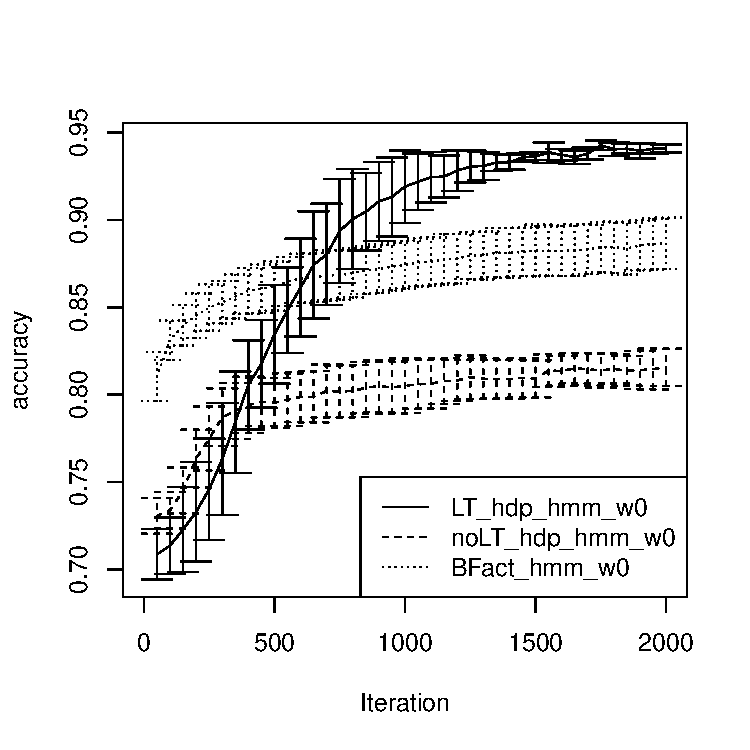
\includegraphics[width = \textwidth]{fig/cocktail_s16_m12/w0/h10.0_nocs_cp1/accuracy.pdf}
\end{minipage}
\hspace{0.1in}
\begin{minipage}{0.40\textwidth}
  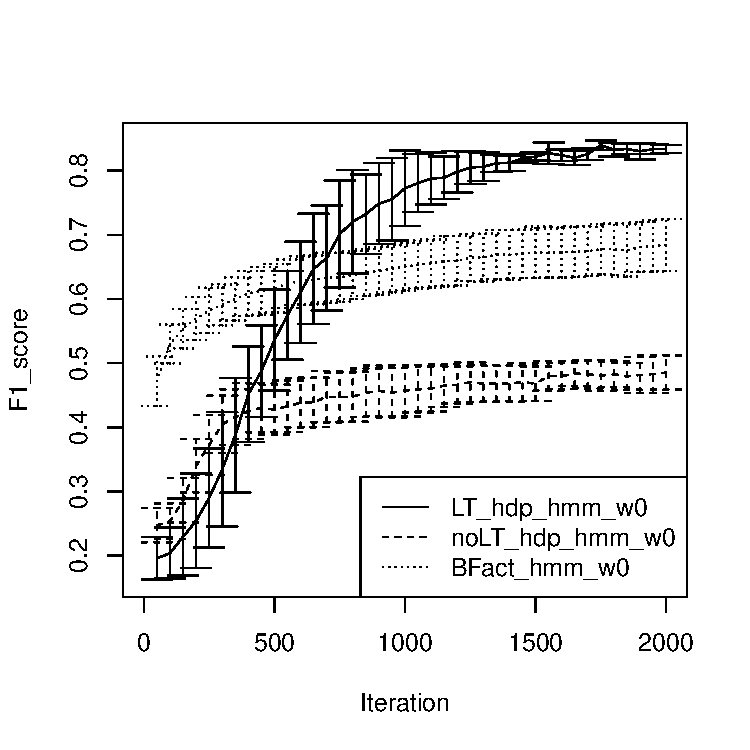
\includegraphics[width = \textwidth]{fig/cocktail_s16_m12/w0/h10.0_nocs_cp1/F1_score.pdf}
\end{minipage}
\vspace{-0.3in}

\begin{minipage}{0.40\textwidth}
  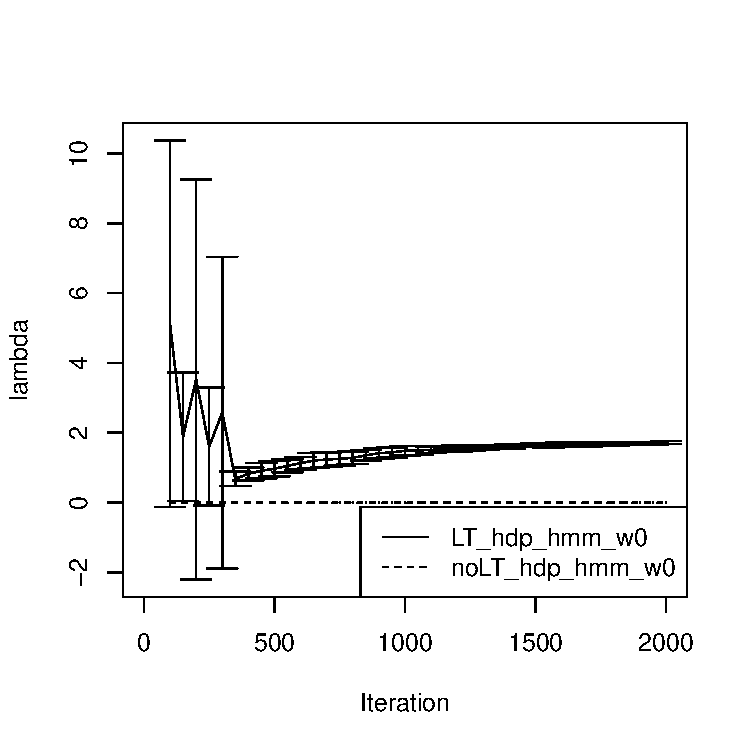
\includegraphics[width = \textwidth]{fig/cocktail_s16_m12/w0/h10.0_nocs_cp1/lambda.pdf}
\end{minipage}
\begin{minipage}{0.40\textwidth}
  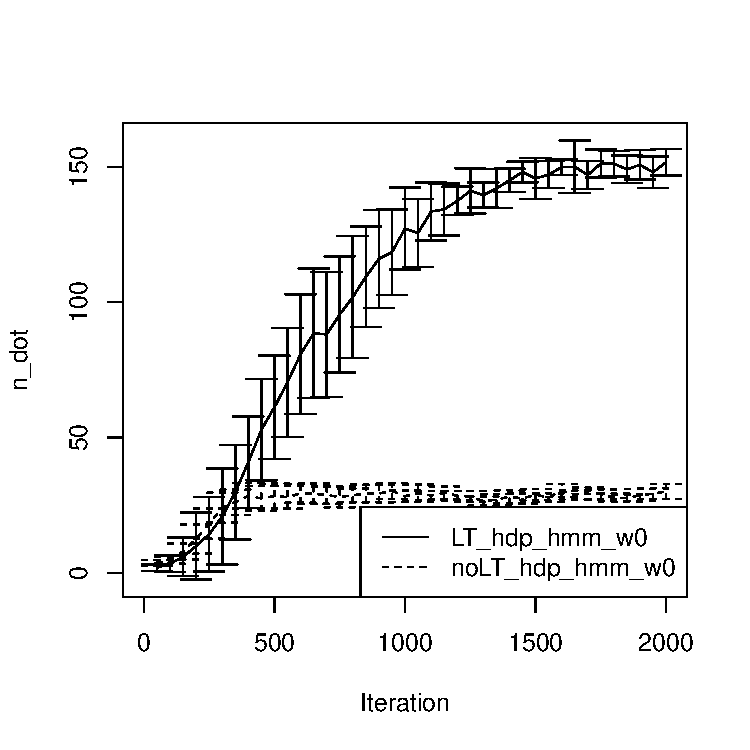
\includegraphics[width = \textwidth]{fig/cocktail_s16_m12/w0/h10.0_nocs_cp1/n_dot.pdf}
\end{minipage}
\caption{(a-b) Accuracy and F1 scores for the HDP-HMM-LT, standard HDP-HMM, and
    Binary Factorial HMM on
    the Cocktail Party Data.  Metrics are averaged
  over 10 Gibbs runs on each model, with error bars representing a 99\% confidence
  interval for the mean per iteration.  The first 100 iterations are
  not shown. (c) Learned similarity parameter, $\lambda$, for the LT
  model, (d) Number of distinct states used by HDP-HMM and
  HDP-HMM-LT.  The first 100 iterations are excluded.}
  \label{fig:cocktail-results}
\end{figure}

\subsection{Synthetic Data Without Local Transitions}
\label{sec:synth-data-without}

We also generated data from an ordinary HDP-HMM, with no local
transition property, in order to investigate the performance of our
model in a case where the data did not have the key property that its
prior equipped it to discover.  The results are in
Fig. \ref{fig:synthetic-results}.
While the $\lambda$ parameter is large, the LT model has worse
performance than the non-LT model on this data, as its bias toward
local transitions is not helpful; however, the
$\lambda$ parameter settles near zero as the model learns that local transitions are not more
probable.  When $\lambda = 0$, the HDP-HMM-LT is an ordinary HDP-HMM.
Unlike on the cocktail party data, the LT model does not use more
states when the data does not have the LT property.

\begin{figure}[tb]
  \centering
  \begin{minipage}{0.40\textwidth}
  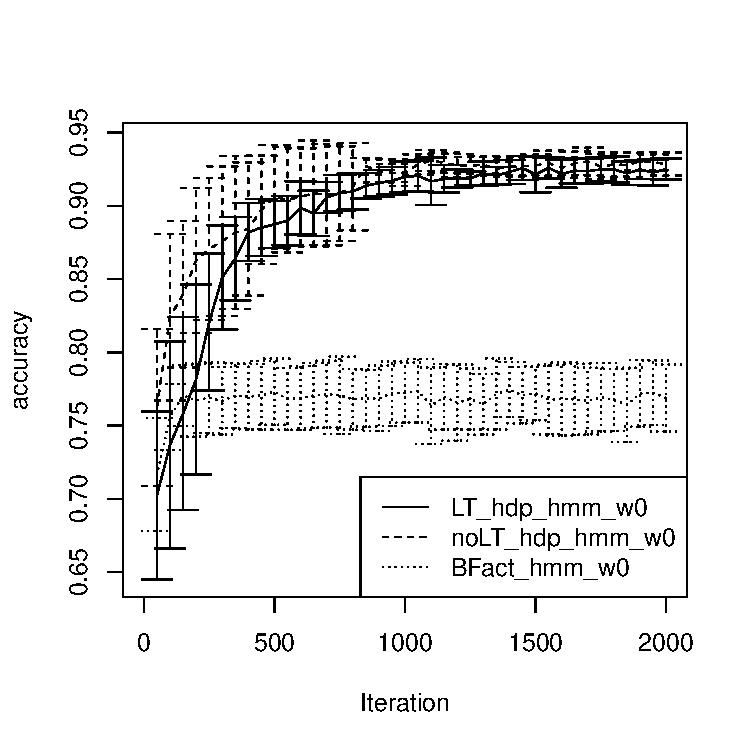
\includegraphics[width =
  \textwidth]{fig/synth16/w0/noLT_s0/accuracy.pdf}
\end{minipage}
\hspace{0.1in}
  \begin{minipage}{0.40\textwidth}
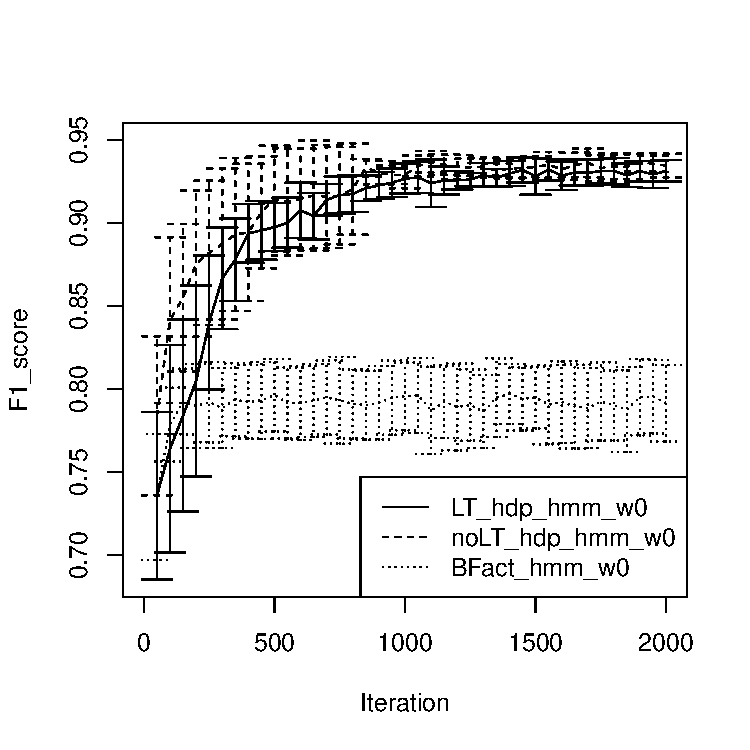
\includegraphics[width = \textwidth]{fig/synth16/w0/noLT_s0/F1_score.pdf}
\end{minipage}

\vspace{-0.3in}

  \begin{minipage}{0.40\textwidth}
  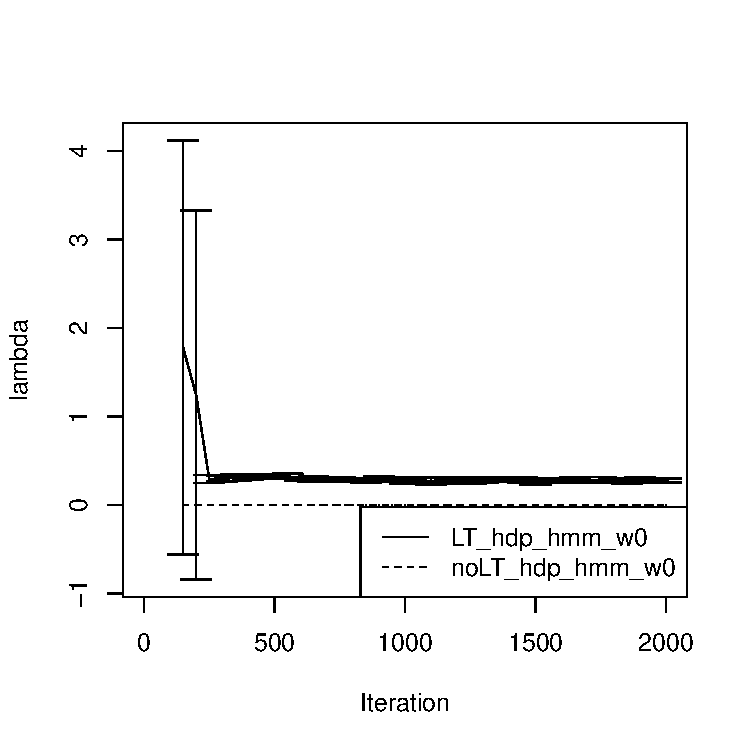
\includegraphics[width = \textwidth]{fig/synth16/w0/noLT_s0/lambda.pdf}
\end{minipage}
  \begin{minipage}{0.40\textwidth}
  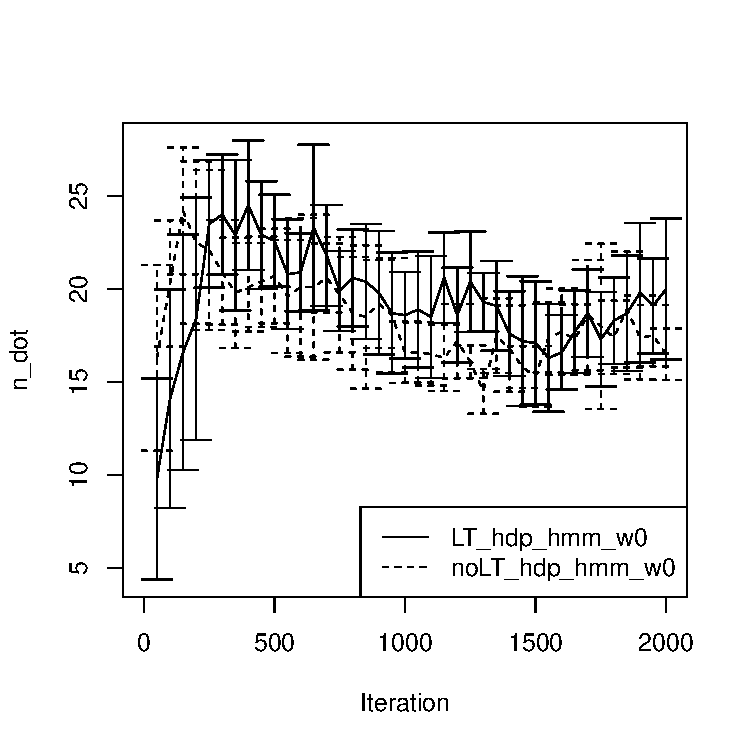
\includegraphics[width = \textwidth]{fig/synth16/w0/noLT_s0/n_dot.pdf}
\end{minipage}
  \caption{(a-b) Accuracy and F1 for the three models on data generated 
    from an HDP-HMM without local transitions, (c) Learned similarity
    parameter, $\lambda$,
  for the LT model, (d) Number of states used by
  the HDP-HMM and HDP-HMM-LT.  The first 100 iterations are omitted.}
  \label{fig:synthetic-results}
\end{figure}

% \begin{figure}[tb]
%   \centering
%   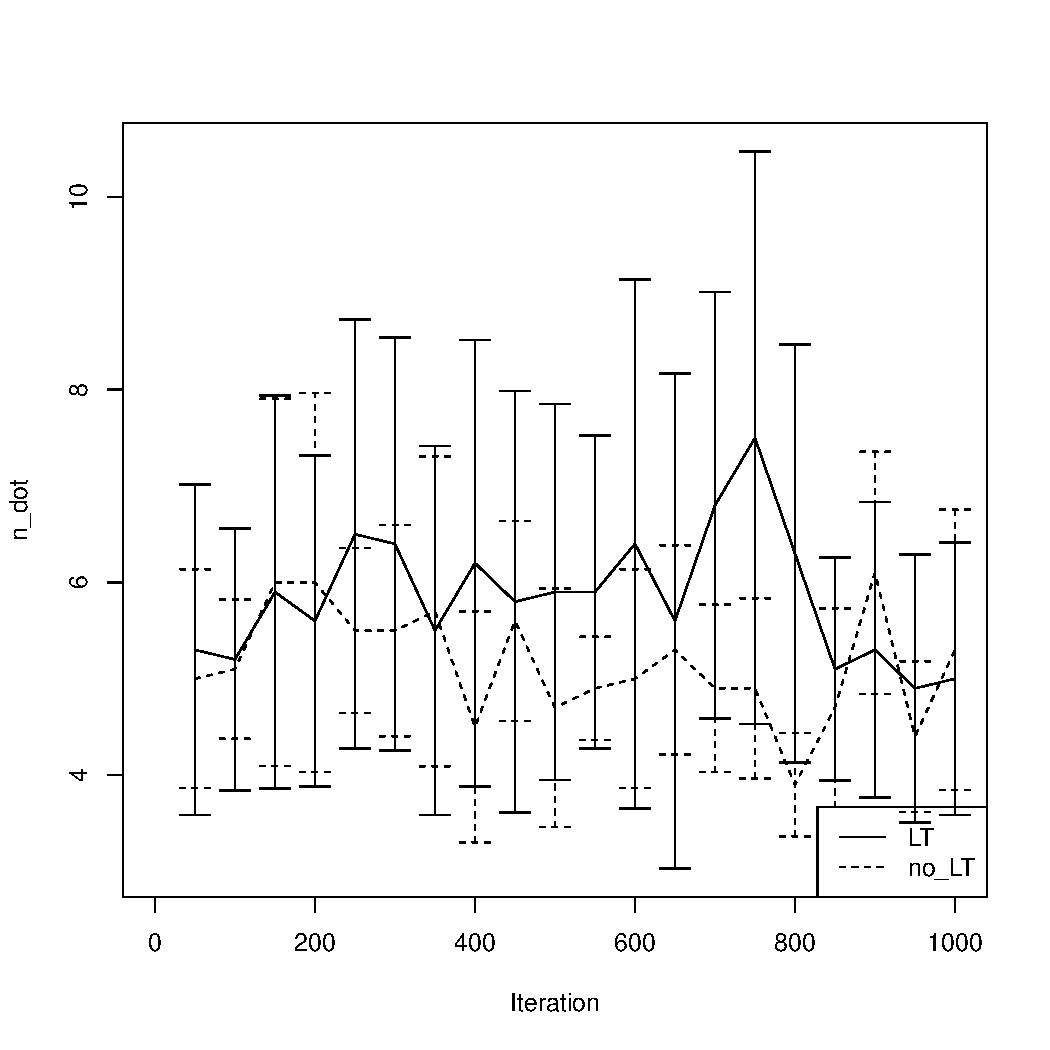
\includegraphics[width = 0.3\textwidth]{fig/synthetic/n_dot}
%   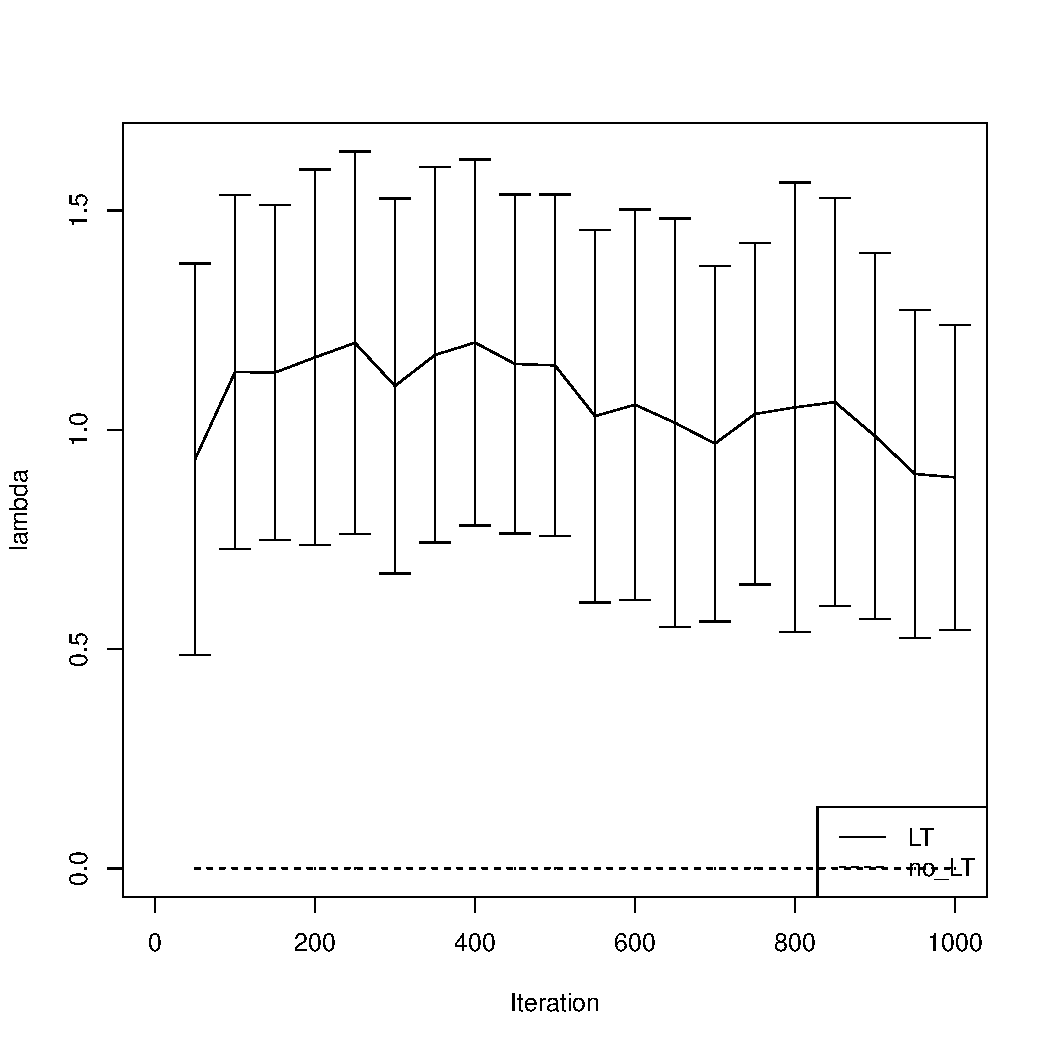
\includegraphics[width = 0.3\textwidth]{fig/synthetic/lambda}
%   \caption{Number of states used on the training data (top), and
%     learned decay rate for the LT model (bottom) on the HDP-HMM data. The first 100
%     iterations are excluded.}
%   \label{fig:synthetic-sparsity}
% \end{figure}
